% vim:autoindent:set textwidth=78:

\section{Panoramica sulle caratteristiche}\label{feature_glance}

% when the revision of a section has been finalized, 
% comment out the following line:
%\updatedisclaimer

Dopo un primo sguardo e una semplice sessione d'esempio nella Sezione \ref{label_getstarted},
forniamo in questo capitolo una panoramica maggiormente dettagliata delle caratteristiche di QGIS. 
Molte delle caratteristiche presentate nei successivi capitoli saranno spiegate
e descritte nelle apposite sezioni del manuale.

\subsection{Avvio e chiusura di QGIS}\label{label_startinqgis}

Nella sezione \ref{samplesession} abbiamo già imparato come avviare QGIS. Ripeteremo 
questa operazione qui per mostrare come QGIS fornisca ulteriori opzioni all'avvio da riga di comando. 

\begin{itemize}
\item \nix{Assumendo che QGIS sia installato nel vostro PATH, si può avviare QGIS 
digitando: \usertext{qgis}  al prompt dei comandi o facendo doppio click sul
collegamento all'applicazione (o allo shortcut) sul desktop o nel menu delle applicazioni.} 
\item \win{Avviare QGIS usando il menu Avvio (Start) o il collegamento sul desktop, 
o facendo doppio click su un progetto QGIS precedentemente salvato.}
\item \osx{Fare doppio click sull'icona QGIS nella cartella Applicazioni (Applications). Se si vuole avviare QGIS
in una shell, eseguire /percorso-installatione-eseguibile/Contents/MacOS/Qgis.}
\end{itemize} 

Per uscire da QGIS, cliccare sul menu \{\nix{}\win{File} \osx{QGIS}\} > Esci,
o usate la scorciatoia da tastiera \keystroke{Ctrl+Q}.

\subsubsection{Opzioni da linea di comando}\index{opzioni da linea di comando}
\label{label_commandline}

\nix QGIS supporta un certo numero di opzioni se avviato da riga di comando.
Per avere una lista delle opzioni possibili, digitare \usertext{qgis ---help} al prompt dei comandi.
La sintassi d'uso di QGIS è:

\small
\begin{verbatim}
qgis --help
Quantum GIS - 1.3.0-Mimas 'Mimas' (exported)
Quantum GIS (QGIS) is a viewer for spatial data sets, including
raster and vector data.
Usage: qgis [options] [FILES]
  options:
        [--snapshot filename]           emit snapshot of loaded datasets to given file
        [--width width]                 width of snapshot to emit
        [--height height]               height of snapshot to emit
        [--lang language]               use language for interface text
        [--project projectfile]         load the given QGIS project
        [--extent xmin,ymin,xmax,ymax]  set initial map extent
        [--nologo]                      hide splash screen
        [--help]                        this text

  FILES:
    Files specified on the command line can include rasters,
    vectors, and QGIS project files (.qgs):
     1. Rasters - Supported formats include GeoTiff, DEM
        and others supported by GDAL
     2. Vectors - Supported formats include ESRI Shapefiles
        and others supported by OGR and PostgreSQL layers using
        the PostGIS extension
\end{verbatim}
\normalsize

\begin{Tip} \caption{\textsc{Esempio di utilizzo delle opzioni da riga di comando}}
\qgistip{QGIS può essere avviato specificando uno o più files da riga di comando.
Per esempio, assunto che ci si trovi nella directory qgis\_sample\_data, 
si può avviare QGIS con un layer vettoriale e un file raster inserendo il seguente comando:
\usertext{qgis ./raster/landcover.img ./gml/lakes.gml}
}
\end{Tip}

\minisec{Opzione da linea di comando \usertext{---snapshot}}
L'opzione consente di creare uno snapshot in formato PNG della vista corrente.
Questo può essere utile quando si hanno molti progetti e si vogliono
generare schermate dai propri dati.

Il file PNG generato ha una risoluzione di 800x600 pixels. Questa può essere adattata
usando gli argomenti \usertext{---width} e \usertext{---height} da riga di comando. 
Dopo l'opzione \usertext{---snapshot} può essere specificato il nome del file con cui si vuole salvare l'immagine.

\minisec{Opzione da linea di comando \usertext{---lang}}
L'interfaccia di QGIS si presenta nella lingua definita dal setting del locale di sistema.
Se si desidera l'interfaccia in un'altra lingua, può essere specificato all'avvio. Ad esempio:
\usertext{---lang=en} fa sì che QGIS si avvii localizzato in inglese.
Un elenco delle lingue correntemente supportate è fornito all'indirizzo
\url{http://wiki.qgis.org/qgiswiki/TranslatorsCorner} 

\minisec{Opzione da linea di comando \usertext{---project}}
È possibile avviare QGIS anche con un file di progetto. Basta semplicemente
aggiungere l'opzione da riga di comando \usertext{---project} seguita dal percorso e dal nome
del progetto e QGIS si aprirà caricando tutti i layer indicati nel file specificato.

\minisec{Opzione da linea di comando \usertext{---extent}}
Per fare sì che QGIS si avvii visualizzando una specifica porzione di mappa, è necessario
specificare i limiti dell'estensione che si intende visualizzare secondo il seguente ordine,
con ogni valore separato da virgole:

\begin{verbatim}
--extent xmin,ymin,xmax,ymax
\end{verbatim}

\minisec{Opzione da linea di comando \usertext{---nologo}}
Questo argomento da riga di comando nasconde lo splash screen quando QGIS viene avviato.

\subsection{Interfaccia QGIS}\index{finestra principale}
\label{label_qgismainwindow}

All'avvio di QGIS si visualizza l'interfaccia grafica riprodotta dalla seguente immagine  
(i numeri da 1 a 6 negli ovali gialli fanno riferimento alle sei principali aree della
interfaccia come qui specificato):

\begin{figure}[ht]
   \begin{center}
   \caption{Interfaccia grafica di QGIS GUI con dati campione dell'Alaska \nixcaption (KDE)}
	 \label{fig:startup}
   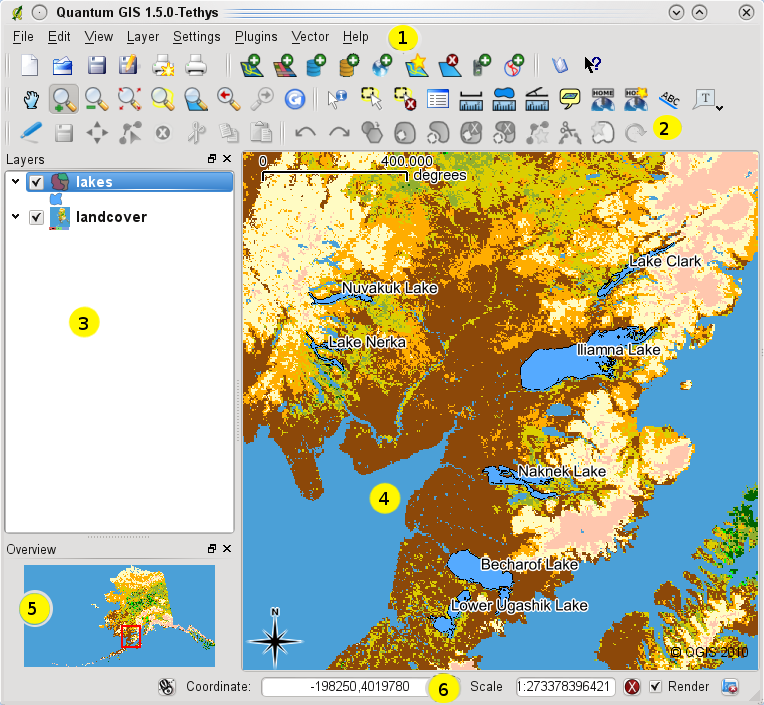
\includegraphics[clip=true, width=17cm]{startup}
\end{center} 
\end{figure}

\textbf{Nota:} L'aspetto delle finestre (barra del titolo, ecc.) può apparire diverso
secondo il sistema operativo e il gestore di finestre adottato.\\

L'interfaccia di QGIS è divisa in sei aree:

\begin{tabbing}
1. Barra Menu \hspace{3cm}\= 4. Vista Mappa \\
2. Barra Strumenti \hspace{3cm}\> 5. Panoramica  \\
3. Legenda \hspace{3cm}\> 6. Barra di Stato   
\end{tabbing}

Le sei componenti dell'interfaccia di QGIS saranno descritte con maggior dettaglio
nelle sezioni seguenti.

\subsubsection{Barra menu}\label{label_menubar}
\index{barra menu}

La barra menu fornisce accesso alle varie caratteristiche di QGIS utilizzando un menu
gerarchico standard. Le voci gerarchicamente più elevate e una sintesi di alcune opzioni
di menu sono elencate di seguito, assieme alle icone dello strumento corrispondente
così come appaiono nella barra strumenti e alle scorciatoie da tastiera per richiamarle.\footnote{Le scorciatoie da tastiera ora possono
essere configurate manualmente (le scorciatoie presentate in questa sezione sono quelle di default), usando lo Strumento Configura 
nel Menu Impostazioni.}
Sebbene molte voci di menu abbiano uno strumento corrispondente e viceversa,
i menu non sono organizzati esattamente come le barre strumenti. 
La barra strumenti che contiene lo strumento descritto è indicata dopo ogni voce di menu
con l'aspetto di una casella di controllo (checkbox).
Per ulteriori informazioni su strumenti e barre degli strumenti, si veda la Sezione \ref{label_toolbars}.

\begin{tabbing}
\hspace{5.5cm}\=\hspace{3cm}\=\hspace{3.5cm}\= \kill
\hspace{1cm} Voce di Menu \> Scorciatoia \> Riferimento \> Barra strumenti\\
\end{tabbing}

\begin{itemize}
\item \mainmenuopt{File}
\begin{tabbing}
\hspace{4.5cm}\=\hspace{3cm}\=\hspace{3.5cm}\= \kill
\dropmenuopttwo{mActionFileNew}{Nuovo progetto}
	\> \keystroke{Ctrl+N}
	\> vedi Sezione \ref{sec:projects}
	\> \dropmenucheck{File} \\
\dropmenuopttwo{mActionFileOpen}{Apri progetto}
	\> \keystroke{Ctrl+O}
	\> vedi Sezione \ref{sec:projects}
	\> \dropmenucheck{File} \\
\dropmenuopt{Apri progetti recenti}
	\>
	\> vedi Sezione \ref{sec:projects} \\
\dropmenuopttwo{mActionFileSave}{Salva progetto}
	\> \keystroke{Ctrl+S}
	\> vedi Sezione \ref{sec:projects}
	\> \dropmenucheck{File} \\
\dropmenuopttwo{mActionFileSaveAs}{Salva progetto con nome}
	\> \keystroke{Ctrl+Shift+S}
  \> vedi Sezione \ref{sec:projects}
	\> \dropmenucheck{File} \\
\dropmenuopttwo{mActionSaveMapAsImage}{Salva come immagine}
	\>
	\> vedi Sezione \ref{sec:output} \\
\dropmenuopttwo{mActionFilePrint}{Compositore stampe}
	\> \keystroke{Ctrl+P}
	\> vedi Sezione \ref{label_printcomposer}
	\> \dropmenucheck{File} \\
\dropmenuopttwo{mActionFileExit}{Esci} 
	\> \keystroke{Ctrl+Q} \\
\end{tabbing}

\item \mainmenuopt{Modifica}
\begin{tabbing}
\hspace{4.5cm}\=\hspace{3cm}\=\hspace{3.5cm}\= \kill
\dropmenuopttwo{mActionUndo}{Annulla}
        \> \keystroke{Ctrl+Z}
        \> vedi Sezione \ref{sec:edit_existing_layer}
        \> \dropmenucheck{Digitalizza} \\
\dropmenuopttwo{mActionRedo}{Ripristina}
        \> \keystroke{Ctrl+Shift+Z}
        \> vedi Sezione \ref{sec:edit_existing_layer}
        \> \dropmenucheck{Digitalizza} \\
\dropmenuopttwo{mActionEditCut}{Taglia geometrie} 
	\> \keystroke{Ctrl+X}
	\> vedi Sezione \ref{sec:edit_existing_layer} 
	\> \dropmenucheck{Digitalizza} \\
\dropmenuopttwo{mActionEditCopy}{Copia geometrie}
	\> \keystroke{Ctrl+C}
	\> vedi Sezione \ref{sec:edit_existing_layer} 
	\> \dropmenucheck{Digitalizza} \\
\dropmenuopttwo{mActionEditPaste}{Incolla geometrie} 
	\> \keystroke{Ctrl+V}
	\> vedi Sezione \ref{sec:edit_existing_layer} 
	\> \dropmenucheck{Digitalizza} \\
\dropmenuopttwo{mActionCapturePoint}{Inserisci punto}
	\> \keystroke{.}
	\> vedi Sezione \ref{sec:edit_existing_layer} 
	\> \dropmenucheck{Digitalizza} \\
\dropmenuopttwo{mActionCaptureLine}{Inserisci linea}
	\> \keystroke{/}
	\> vedi Sezione \ref{sec:edit_existing_layer} 
	\> \dropmenucheck{Digitalizza} \\
\dropmenuopttwo{mActionCapturePolygon}{Inserisci poligono}
	\> \keystroke{Ctrl+/}
	\> vedi Sezione \ref{sec:edit_existing_layer} 
	\> \dropmenucheck{Digitalizza} \\
E altre voci del menu Modifica
	\>
	\> vedi Sezione \ref{sec:edit_existing_layer} 
	\> \dropmenucheck{Digitalizza} \\
%\dropmenuopt{Move Feature}
%	\> \> \dropmenucheck{Edit} \\
%\dropmenuopt{Split Features}
%	\> \> \dropmenucheck{Edit} \\
%\dropmenuopt{Delete Selected}
%	\> \> \dropmenucheck{Edit} \\
%\dropmenuopt{Add Vertex}
%	\> \> \dropmenucheck{Edit} \\
%\dropmenuopt{Move Vertex}
%	\> \> \dropmenucheck{Edit} \\
%\dropmenuopt{Delete Vertex}
%	\> \> \dropmenucheck{Edit} \\
%\dropmenuopt{Add Ring}\footnote{New since v0.9} 
%	\>
%	\> \dropmenucheck{Edit} \\
%\dropmenuopt{Add Island} \footnotemark[\value{footnote}] 
%	\>
%	\> \dropmenucheck{Edit} \\
\end{tabbing}


\item \mainmenuopt{Visualizza}
\begin{tabbing}
\hspace{4.5cm}\=\hspace{3cm}\=\hspace{3.5cm}\= \kill
\dropmenuopttwo{mActionPan}{Sposta mappa}
	\>
	\> \> \dropmenucheck{Navigazione mappa} \\
\dropmenuopttwo{mActionZoomIn}{Ingrandisci}
	\> \keystroke{Ctrl++}
	\> \> \dropmenucheck{Navigazione mappa} \\
\dropmenuopttwo{mActionZoomOut}{Rimpicciolisci}
	\> \keystroke{Ctrl+-}
	\> \> \dropmenucheck{Navigazione mappa} \\
\dropmenuopttwo{mActionSelect}{Seleziona geometrie}
	\>
	\> \> \dropmenucheck{Attributi} \\
\dropmenuopttwo{mActionIdentify}{Informazioni geometrie}
	\> \keystroke{I}
	\> \> \dropmenucheck{Attributi} \\
\dropmenuopttwo{mActionMeasure}{Misura linea}
	\> \keystroke{M}
	\> \> \dropmenucheck{Attributi} \\
\dropmenuopttwo{mActionMeasureArea}{Calcola l'area}
	\> \keystroke{J}
	\> \> \dropmenucheck{Attributi} \\
\dropmenuopttwo{mActionOpenTable}{Vista massima}
	\> \keystroke{F}
	\> \> \dropmenucheck{Navigazione mappa} \\
\dropmenuopttwo{mActionZoomToLayer}{Zoom sul layer}
	\>
	\> \> \dropmenucheck{Navigazione mappa} \\
\dropmenuopttwo{mActionZoomToSelected}{Zoom sulla selezione}
	\> \keystroke{Ctrl+J}
	\> \> \dropmenucheck{Navigazione mappa} \\
\dropmenuopttwo{mActionZoomLast}{Ultimo zoom}
	\>
	\> \> \dropmenucheck{Navigazione mappa} \\
\dropmenuopttwo{mActionZoomNext}{Prossimo zoom}
	\>
	\> \> \dropmenucheck{Navigazione mappa} \\
\dropmenuopt{Zoom dimensione corrente}
	\>
	\> \>  \\
\dropmenuopttwo{mActionMapTips}{Suggerimenti mappa}
	\>
	\> \> \dropmenucheck{Attributi} \\
\dropmenuopttwo{mActionNewBookmark}{Nuovo segnalibro}
	\> \keystroke{Ctrl+B}
	\> vedi Sezione \ref{sec:bookmarks} 
\> \dropmenucheck{Attributi} \\
\dropmenuopttwo{mActionShowBookmarks}{Mostra segnalibri}
	\> \keystroke{B}
	\> vedi Sezione \ref{sec:bookmarks} 
	\> \dropmenucheck{Attributi} \\
\dropmenuopttwo{mActionDraw}{Aggiorna}
	\> \keystroke{Ctrl+R}
	\> \> \dropmenucheck{Navigazione mappa} \\
\end{tabbing}

\item \mainmenuopt{Layer}
\begin{tabbing}
\hspace{5cm}\=\hspace{3cm}\=\hspace{3.5cm}\= \kill
\dropmenuopttwo{mActionNewVectorLayer}{Nuovo layer vettoriale}
	\> \keystroke{N}
	\>          	
	vedi Sezione \ref{sec:create shape}
	\> \dropmenucheck{Gestisci layer} \\
\dropmenuopttwo{mActionAddNonDbLayer}{Aggiungi layer vettoriale}       
	\> \keystroke{V}
	\>          	
	vedi Sezione \ref{label_workingvector}
	\> \dropmenucheck{File} \\
\dropmenuopttwo{mActionAddRasterLayer}{Aggiungi layer raster}       
	\> \keystroke{R}
	\>          	
	vedi Sezione \ref{label_raster}
	\> \dropmenucheck{File} \\
\dropmenuopttwo{mActionAddLayer}{Aggiungi layer PostGIS}      
	\> \keystroke{D}
	\>          	
	vedi Sezione \ref{label_postgis}
        \> \dropmenucheck{File} \\
\dropmenuopttwo{mActionAddSpatiaLiteLayer}{Aggiungi layer SpatiaLite}
        \> \keystroke{L}
        \>
        vedi Sezione \ref{label_spatialite}
	\> \dropmenucheck{File} \\
\dropmenuopttwo{mActionAddWmsLayer}{Aggiungi layer WMS}          
	\> \keystroke{W}
	\>          	
	vedi Sezione \ref{sec:ogc-wms}
	\> \dropmenucheck{File} \\
\dropmenuopttwo{mActionOpenTable}{Apri tabella attributi}
	\> \>
	\> \dropmenucheck{Attributi} \\
\dropmenuopttwo{mActionToggleEditing}{Attiva/disattiva modifica}
	\> \>
	\> \dropmenucheck{Digitalizza} \\
\dropmenuopt{Salva come shapefile}
	\\
\dropmenuopt{Salva selezione come shapefile}
	\\
\dropmenuopttwo{mActionRemoveLayer}{Elimina Layer}
	\> \keystroke{Ctrl+D}
	\>          	
	\> \dropmenucheck{Gestisci layer} \\
\dropmenuopt{Proprietà}
	\\
\dropmenuopttwo{mActionInOverview}{Aggiungi alla panoramica}
	\> \keystroke{O}
	\>          	
	\> \dropmenucheck{Gestisci layer} \\
\dropmenuopttwo{mActionAddAllToOverview}{Aggiungi tutto alla panoramica}
	\> \keystroke{+}
	\>          	
	\\
\dropmenuopttwo{mActionRemoveAllFromOverview}{Rimuovi tutto dalla panoramica}
	\> \hspace{1cm}\keystroke{-}
	\>          	
	\\
\dropmenuopttwo{mActionHideAllLayers}{Nascondi tutti i layer}
	\> \keystroke{H}
	\>          	
	\> \dropmenucheck{Gestisci layer} \\
\dropmenuopttwo{mActionShowAllLayers}{Mostra tutti i layer}
	\> \keystroke{S}
	\>          	
	\> \dropmenucheck{Gestisci layer} \\
\end{tabbing}

\item \mainmenuopt{Impostazioni}
\begin{tabbing}
\hspace{4.5cm}\=\hspace{3cm}\=\hspace{3.5cm}\= \kill
\dropmenuopt{Pannelli}  
	\>           
	\>          	
	\\
\dropmenuopt{Barre degli strumenti}  
	\>           
	\>          	
	\\
\dropmenuopt{Attiva/Disattiva schermo intero}  
	\>
	\>          	
	\\
\dropmenuopttwo{mActionProjectProperties}{Proprietà progetto}  
	\> \keystroke{P}
	\> vedi Sezione \ref{sec:projects}
	\\
\dropmenuopttwo{mActionCustomProjection}{CRS personalizzato}   
\> \> vedi Sezione \ref{sec:customprojections}
	\\
\dropmenuopttwo{mActionOptions}{Configura scorciatoie}
        \>
        \>
        \\
\dropmenuopttwo{mActionOptions}{Opzioni}             
\> \>          	
vedi Sezione \ref{subsec:gui_options}
	\\
\end{tabbing}

\item \mainmenuopt{Plugins} - (Ulteriori voci di menu vengono aggiunte quando si installano e caricano nuovi plugin.)
\begin{tabbing}
\hspace{4.5cm}\=\hspace{3cm}\=\hspace{3.5cm}\= \kill
\dropmenuopttwo{mActionShowPluginManager}{Gestione Plugins}          	 
	\> \> vedi Sezione \ref{sec:managing_plugins} \dropmenucheck{Plugin}
	\\
	\dropmenuopt{Python Console}
        \> \>
        \\
\end{tabbing}          	

\item \mainmenuopt{Aiuto}
\begin{tabbing}
\hspace{4.5cm}\=\hspace{3cm}\=\hspace{3.5cm}\= \kill
\dropmenuopttwo{mActionHelpContents}{Aiuto contenuti}
	\> \keystroke{F1}
	\>           	
	\> \dropmenucheck{Aiuto}\\
\dropmenuopttwo{mActionQgisHomePage}{QGIS Home Page}
	\> \keystroke{Ctrl+H}
	\>          	
	\\
\dropmenuopttwo{mActionCheckQgisVersion}{Controlla versione QGIS}
	\\
\dropmenuopttwo{mActionHelpAbout}{Informazioni}
	\\
\end{tabbing}

\end{itemize}

\textbf{Nota:} \nix Gli elementi della barra menu elencati di seguito sono quelli di default nel gestore finestre di KDE. 
In GNOME il menu Impostazioni non è presente e i suoi elementi devono essere cercati
qui:
\begin{tabbing}
\dropmenuopttwo{mActionProjectProperties}{Project Properties} \hspace{3cm}\=
\dropmenucheck{File menu} \\
\dropmenuopttwo{mActionOptions}{Options} \hspace{3cm}\>
\dropmenucheck{Edit}\\
\dropmenuopttwo{mActionCustomProjection}{Custom CRS}\hspace{3cm}\>
\dropmenucheck{Edit} \\
\dropmenuopt{Panels} \hspace{3cm}\>
\dropmenucheck{View} \\
\dropmenuopt{Toolbars}   \hspace{3cm}\>
\dropmenucheck{View} \\
\dropmenuopt{Toggle Fullscreen Mode} \hspace{3cm}\>
\dropmenucheck{View}
\end{tabbing}

%See Appendix \ref{app_menu} for complete descriptions of the menu items.

\subsubsection{Barre degli strumenti}\label{label_toolbars}
\index{barre degli strumenti}

Le barre degli strumenti forniscono accesso alla maggior parte delle medesime funzioni presenti nei menu,
oltre a funzioni addizionali per interagire con la mappa. Ogni oggetto della barra strumenti
ha disponibile un aiuto a comparsa. Lasciando il cursore del mouse sopra l'icona verrà
visualizzata una breve descrizione della funzione fornita da quello strumento.

Ogni barra può essere spostata secondo le preferenze personali. Inoltre ognuna di esse
può essere disattivata dal menu contestuale ottenibile cliccando con il tasto destro
sulla barra degli strumenti.

\begin{Tip}
\caption{\textsc{Ripristinare barre degli strumenti}} \index{disposizione!barre degli strumenti}
\qgistip{Se avete accidentalmente disattivato tutte le barre strumenti,
possono essere ripristinate dalla voce di menu \mainmenuopt{Impostazioni} > \dropmenuopt{Barre degli strumenti}.}
\end{Tip}

\subsubsection{Legenda}\label{label_legend}
\index{legenda}

L'area di legenda è usata per impostare la visibilità e l'ordine di sovrapposizione dei layer:
i layer in cima alla legenda coprono nella mappa quelli sottostanti.
La casella di controllo in ogni legenda può essere usata per attivare/disattivare la 
visibilità di un layer.\index{layer!visibilità}

È possibile raggruppare layer nella legenda aggiungendo un gruppo e trascinando i layer nel gruppo.
Per fare ciò cliccare con il tasto destro nell'area di legenda, scegliere \dropmenuopt{Aggiungi gruppo}. 
Apparirà una nuova cartella nella quale possono essere trascinati i layer che si intendono raggruppare. È quindi possibile attivare/disattivare la 
visibilità di tutti i layer nel gruppo con un solo click. Per estrarre un layer dal gruppo, muovere 
il puntatore del mouse sul simbolo del layer, cliccare con il tasto destro e scegliere \dropmenuopt{Crea all'oggetto in cima}. Per rinominare il gruppo, 
fare click con il tasto destro sulla cartella e scegliere \dropmenuopt{Rinomina} dal menu contestuale.

Il contenuto del menu contestuale varia a seconda che si faccia click col tasto destro
su un layer raster o vettoriale. Per i layer vettoriali di GRASS la voce di menu \dropmenuopt{Attiva/disattiva modifica}
non è abilitata. Si veda la sezione \ref{grass_digitising} per informazioni su come editare layer vettoriali GRASS. 

\begin{itemize}

\item \textbf{Menu relativo ai raster attivabile con il tasto destro del mouse}
\begin{itemize}
\item \dropmenuopt{Zoom all'estensione del layer}
\item \dropmenuopt{Zoom alla scala migliore (100\%)}
\item \dropmenuopt{Aggiungi alla panoramica}
\item \dropmenuopt{Rimuovi}
\item \dropmenuopt{Proprietà}
\item \dropmenuopt{Rinomina}
\item \dropmenuopt{Aggiungi gruppo}
\item \dropmenuopt{Espandi tutto}
\item \dropmenuopt{Comprimi tutto}
\item \dropmenuopt{Mostra gruppi}
\end{itemize}

\item \textbf{Menu relativo ai vettoriali attivabile con il tasto destro del mouse}
\begin{itemize}
\item \dropmenuopt{Zoom all'estensione del layer}
\item \dropmenuopt{Aggiungi alla panoramica}
\item \dropmenuopt{Rimuovi}
\item \dropmenuopt{Apri tabella attributi}
\item \dropmenuopt{Attiva/disattiva modifica (non disponibile per layer GRASS)}
\item \dropmenuopt{Salva come shapefile}
\item \dropmenuopt{Salva selezione come shapefile}
\item \dropmenuopt{Proprietà}
%% \item \dropmenuopt{Crea all'oggetto in cima}
\item \dropmenuopt{Rinomina}
\item \dropmenuopt{Aggiungi gruppo}
\item \dropmenuopt{Espandi tutto}
\item \dropmenuopt{Comprimi tutto}
\item \dropmenuopt{Mostra gruppi}
\end{itemize}

\item \textbf{Menu relativo ai gruppi di layer attivabile con il tasto destro del mouse} 
\begin{itemize}
\item \dropmenuopt{Rimuovi}
\item \dropmenuopt{Rinomina}
\item \dropmenuopt{Aggiungi gruppo}
\item \dropmenuopt{Espandi tutto}
\item \dropmenuopt{Comprimi tutto}
\item \dropmenuopt{Mostra gruppi}
\end{itemize}

\end{itemize}

Se diversi vettori hanno lo stesso tipo di geometria e gli stessi attributi le loro proprietà di visualizzazione
possono essere raggruppate. Questo significa che se la proprietà di visualizzazione di un
layer è cambiata automaticamente gli altri prenderanno lo stesso tipo di visualizzazione. Per raggruppare
la simbologia scegli la voce \dropmenuopt{Mostra gruppi} dal menu contestuale dei "Gruppi di layer" e sarà
possibile trascinare i file da un file di gruppo ad un un altro. Se questo verrà fatto la simbologia sarà
raggruppata. Nota che QGIS permette di spostare i file di gruppo solo se i due layer sono compatibili
(stesso geometria e stessi attributi).

%% isn't included in Titan anymore, except for an "toggle overview"
%Each legend entry can show the following mini icons:
%
%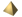
\includegraphics[width=0.7cm]{pyramid} This is a raster
%that has pyramids built for it to improve rendering efficiency (see
%Section \ref{raster_pyramids}).\\
%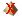
\includegraphics[width=0.7cm]{no_pyramid} This is a
%raster that has no pyramid layers (see Section \ref{raster_pyramids}).\\
%
\includegraphics[width=0.7cm]{inoverview} This layer is
%shown in the overview map area as well as in the main map window.\\
%
\includegraphics[width=0.7cm]{editable} This is a vector
%layer that is currently enabled for editing.\\

\subsubsection{Il visualizzatore di mappa}\label{label_mapview}
\index{mappa!vista}

Questa è l’area in cui le mappe vengono visualizzate. La mappa visualizzata in questa finestra sarà
il risultato dei layer vettoriali e raster che avete scelto di caricare (vedere le sezioni che seguono
per ulteriori informazioni su come caricare i layer). La zona di visualizzazione della mappa può
essere modificata (spostando la messa a fuoco dell’esposizione della mappa ad un’altra regione) ed
è possibile effettuare operazioni di zoom in ed out (+ e -). Varie altre operazioni sono descritte nella
sezione relativa alla barra dei menu. La vista nell’area di mappa e la legenda sono strettamente
legate l’una all’altra: le mappe che vengono visualizzate riflettono i cambiamenti che fate nella zona
della legenda.  

\begin{Tip}\caption{\textsc{Zoomare rapidamente con la rotella del mouse}}\index{zoom!rotella mouse}
\qgistip{Può essere usata la rotella del mouse per le operazioni di zoom.
Posizionando il puntatore nell'area di visualizzazione delle mappe si aumenta
lo zoom girando la rotella verso lo schermo, lo si riduce girandola verso di
sé. La posizione del puntatore costituisce il centro per l'ingrandimento. Il
comportamento della funzione di zoom con la rotella del mouse può essere
regolata dalla scheda \tab{Strumenti di mappa} sotto il menu
\mainmenuopt{Impostazioni} >\dropmenuopt{Opzioni}.  }
\end{Tip}

\begin{Tip}\caption{\textsc{Muovere la mappa con i tasti freccia e la barra spaziatrice}}\index{muovere la mappa!tasti freccia}
\qgistip{È possibile usare i tasti freccia per muovere la mappa. Posizionando il puntatore del mouse 
nell'area di visualizzazione delle mappe, ci si muove verso Est con la freccia destra, 
verso Ovest con quella sinistra, verso Nord con la freccia Sù e verso Sud con la freccia Giù. 
Si può spostare la mappa anche tenendo premuta la barra spaziatrice e
muovendo il mouse.
}
\end{Tip}

\subsubsection{Panoramica della mappa}\label{label_mapoverview}
\index{mappa!panoramica}

Il pannello di panoramica della mappa fornisce una vista completa dei layer aggiunti ad essa. Può 
esssere selezionato nel menu \mainmenuopt{Impostazioni}. >\dropmenuopt{Pannelli}.
All’interno della panoramica c’è un rettangolo che mostra l’estensione corrente della mappa. Ciò permette 
di determinare rapidamente quale area della mappa state attualmente osservando. Si noti 
che le etichette non sono visualizzate nella panoramica della mappa anche se i layer 
hanno la funzione di visualizzazione delle etichette attiva labeling. 

Può essere aggiunto un singolo layer alla panoramica facendo click col tasto destro su di 
esso nella legenda e scegliendo poi \checkbox{Aggiungi alla panoramica}. Possono anche essere aggiunti o rimossi tutti i layer nella
panoramica usando lo strumento "Panoramica" nella barra degli strumenti. 

Cliccando e trascinando nella panoramica il rettangolo rosso che mostra
l'estensione corrente della vostra visuale, la mappa visualizzata si sposta di conseguenza.

\subsubsection{Barra di stato}\label{label_statusbar}

La barra di stato mostra la posizione del cursore attuale nella mappa nelle
coordinate specificate (es. metri o gradi decimali).
Nella barra di stato a sinistra del visore delle coordinate è presente un
piccolo pulsante che consente di passare dalla visione delle coordinate al
movimento del puntatore a
quella dell'estensione della vista quando si effettua lo zoom.

Una barra di avanzamento nella barra di stato mostra il progredire della
visualizzazione di ogni layer nella vista mappa. In alcuni casi, come quando
vengono raccolte informazioni statistiche sul layer raster, questa barra è
utilizzata per mostrare lo stato di tali processi, in genere molto lunghi. 

Se è disponibile un nuovo plugin o un aggiornamento ad un plugin installato,
nella barra di stato apparirà un avviso. Sulla destra della barra di stato è
presente una casella di controllo (checkbox) che può essere usata per
disattivare temporaneamente la visualizzazione dei layer nella vista (vedi
Sezione \ref{subsec:redraw_events} più avanti). All'estrema destra della barra
di stato è presente l'icona di un proiettore. Cliccando su di essa si apre la
finestra con le proprietà della proiezione del progetto corrente.

\begin{Tip}\caption{\textsc{Calcolare la scala corretta della mappa}}\index{scala!calcolare}
\qgistip{Quando si avvia QGIS, l'unità di default sono i gradi, il che fa si
che QGIS interpreti ogni coordinata del layer in gradi. Per avere il corretto
valore della scala, è possibile sia cambiare manualmente l'unità di misura a
metri nella scheda \tab{Generale} sotto 
il menu \mainmenuopt{Impostazioni} >\dropmenuopt{Proprietà progetto} oppure può essere scelto un Sistema
di Riferimento per le Coordinate (Coordinate Reference System, CRS), cliccando
sull'icona \toolbtntwo{mIconProjectionDisabled}{Stato CRS} 
nell'angolo in basso a destra della barra di stato. In quest'ultimo caso, le 
unità della mappa sono impostate a quelle che specifica la proiezione scelta, ad es. "+units=m".
}
\end{Tip}

\subsection{Visualizzazione}\label{subsec:redraw_events}\index{visualizzazione}

Come impostazione di default QGIS ricarica nella vista tutti i layer visibili
ogni qualvolta la vista debba essere aggiornata. Gli eventi che richiedono
l'aggiornamento della vista includono:

\begin{itemize}
\item Aggiunta di un layer
\item Spostamento, ingrandimento o riduzione
\item Ridimensionamento della finestra di QGIS
\item Cambiamento della visibilità di uno o più layer
\end{itemize}

QGIS consente di controllare il processo di resa a video in diverse maniere.

\subsubsection{Visualizzazione in funzione della scala}\index{visualizzazione!in funzione della scala}
\label{label_scaledepend}

La visualizzazione in funzione della scala consente di specificare la scala
minima e massima rispettivamente al di sotto e al di sopra della quale un
layer è visibile. Per impostare la visualizzazione in funzione della scala,
aprire la finestra di dialogo \dialog{Proprietà} facendo doppio click sul
layer nella legenda. Nella scheda \tab{Generale}, spuntare la casella di
controllo \checkbox{Utilizzare una scala in relazione al rendering} e impostare i valori per la scala minima e massima.

I valori di scala possono essere determinati usando prima lo zoom sul layer per
il quale si vuole impostare l'opzione e prendendo successivamente nota del valore di scala
visualizzato nella barra di stato di QGIS.\index{scala}

\subsubsection{Controllo della resa a video della mappa}\label{label_controlmap}

La resa a video mappa può essere controllata nei seguenti modi:

\minisec{a) Sospensione della resa a video}\index{visualizzazione!sospensione}
\label{label_suspendrender}

Per sospendere la resa a video, cliccare sulla casella di controllo
\checkbox{Disegna} in basso a destra della barra di stato. Quando la casella
\checkbox{Disegna} non è selezionata, QGIS non ridisegna la vista quando si
verifica uno degli eventi precedentemente descritti alla Sezione
\ref{subsec:redraw_events}. Casi in cui si potrebbe voler sospendere la
visualizzazione a video includono:

\begin{itemize}
\item Aggiunta di molti layer e applicazione di uno stile visuale prima della
resa
\item Aggiunta di uno o più layer di grosse dimensioni e impostazione di una
scala prima della resa
\item Aggiunta di uno o più layer di grossa dimensione e zoom ad un'area specifica prima della resa
\item Combinazioni delle precedenti
\end{itemize}

Selezionando la casella di controllo \checkbox{Disegna} abilita la resa a
video e causa l'immediata rivisualizzazione della vista mappa.

\minisec{b) Regolazione dell'opzione per controllare la visibilità dei
layer quando sono aggiunti}\label{label_settinglayer}
\index{visualizzazione!opzioni}\index{layer!visualizzazione iniziale}

Può essere scelta l'opzione di caricare i nuovi layer senza che essi vengano
immediatamente resi a video. Ciò significa che quando si aggiungerà un layer
al progetto la casella di controllo per la visibilità nella legenda sarà
disabilitata di default. Per impostare questa opzione, scegliere l'opzione di
menu \mainmenuopt{Impostazioni} > \dropmenuopt{Opzioni} e cliccate sulla
scheda \tab{Disegno}. Deselezionare la casella di controllo \checkbox{Per
impostazione predefinita i nuovi layer aggiunti alla mappa vengono
visualizzati subito}. Ogni layer aggiunto alla mappa sarà quindi spento
(invisibile) di default.

%\minisec{Stopping Rendering}\index{visualizzazione!interruzione}
%\label{label_stoprender}
%
%To stop the map drawing, press the ESC key. This will halt the refresh of
%the map canvas and leave the map partially drawn. It may take a bit of time
%between pressing ESC and the time the map drawing is halted.
%
%\textbf{NOTE}: It is currently not possible to stop rendering - this was disabled 
%in qt4 port because of User Interface (UI) problems and crashes.

\minisec{c) Aggiornamento della mappa durante la visualizzazione}
\label{label_updatemap}\index{visualizzazione!aggiornamento vista}

Può essere impostata un'opzione per aggiornare la mappa man mano che gli
elementi del layer vengono letti. Di default, QGIS non traccia alcun elemento a video
fino a che l'intero layer non sia stato letto. Per aggiornare la visualizzazione
man mano che gli elementi vengono letti dall'archivio, selezionare la
voce di menu \mainmenuopt{Impostazioni} > \dropmenuopt{Opzioni} e cliccare sulla
scheda \tab{Disegno} tab. Impostare il numero di elementi che si desidera
vengano letti prima che lo schermo venga aggiornato. Un valore pari a 0
disabilita l'aggiornamento durante la tracciatura degli oggetti (impostazione
predefinita). Un valore troppo basso diminuisce le prestazioni in quanto la
mappa viene continuamente aggiornata man mano che gli elementi del layer
vengono letti. Il valore di prova suggerito per iniziare è 500. 

\minisec{d) Modificare la qualità della resa a video}
\label{label_renderquality}\index{visualizzazione!qualità}

Vi sono 3 opzioni per modificare la qualità della resa a video. Dal menu
\mainmenuopt{Impostazioni} > \dropmenuopt{Opzioni} cliccare sulla scheda
\tab{Disegno} e selezionare o deselezionare le seguenti caselle di controllo.
\begin{itemize}
\item \checkbox{Rendi le linee meno dettagliate in favore di migliori
prestazioni nel disegno}
\item \checkbox{Risolvi problemi con poligoni riempiti non correttamente}
%%\item \checkbox{Ridisegna la mappa mentre viene spostato il divisore legenda/mappa}
\end{itemize}


\subsection{Misurazioni}\label{sec:measure}\index{misura}

È possibile effettuare misure unicamente nei sistemi di coordinate piani
(es. UTM). Se la mappa caricata è definita in un sistema di coordinate
geografiche (es. latitudine/longitudine), il risultato della misura di linee o
di aree saranno errati. Per misurare è quindi necessario impostare
correttamente il sistema di coordinate della mappa (si veda la Sezione \ref{label_projections}).

\subsubsection{Misurare lunghezze e aree}\index{misura!lunghezza}\index{misura!area}
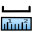
\includegraphics[width=0.7cm]{mActionMeasure} 
QGIS è in grado di fornire la misura di distanza reale tra due punti in
funzione di un definito ellissoide. Ciò può essere configurato dall'opzione di
menu \mainmenuopt{Impostazioni} > \dropmenuopt{Opzioni}, 
cliccando sulla scheda \tab{Strumenti mappa} e scegliendo l'ellissoide
appropriato. Qui sarà possibile inolre definire  a rubberband color e l'unità di misura preferita 
(metri o piedi). Lo strumento consentirà allora di cliccare punti sulla mappa.
La misura di ogni segmento verrà mostrata nella finestra dello strumento insieme alla misura totale. Per terminare la funzione misura cliccare con il
tasto destro del mouse. \\

\includegraphics[width=0.7cm]{mActionMeasureArea} Questo strumento consente la
misura di aree, la finestra mostrerà unicamente l'area totale misurata.
In aggiunta, lo strumento di misura farà lo snap sul layer selezionato al momento, nel caso il layer abbia definita la sua tollezanza di snap. 
(Vedi Sezione~\ref{snapping_tolerance}). 
Se dunque si vuole misurare esattamente lungo una linea o un poligono, è necessario prima definire la sua tolleranza di snap, poi selezionae il layer. 
In questo modo, quando vengono usati gli strumenti di misura, ogni click del mouse (all'interno della tolleranza definita) si aggancerà a quel layer. 

\begin{figure}[h]
\caption{Strumento di misura in azione \nixcaption} \label{fig:measure}
\centering
   \subfigure[Misura linee] {\label{subfig:measure_line}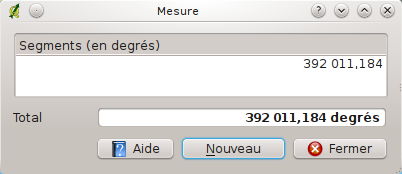
\includegraphics[clip=true, width=0.3\textwidth]{measure_line}}\goodgap
   \subfigure[Misura aree]{\label{subfig:measure_area}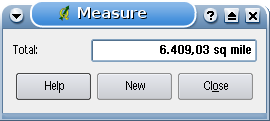
\includegraphics[clip=true, width=0.3\textwidth]{measure_area}}
\end{figure}

\subsection{Progetti}\label{sec:projects}\index{progetti}

Lo stato della sessione QGIS è considerata un progetto. 
È possibile lavorare su un progetto alla volta. Le impostazioni possono essere settate 
per ogni singolo progetto oppure come default per tutti i nuovi progetti (si veda la Sezione
\ref{subsec:gui_options}). Lo stato della sessione corrente può essere salvato
in un progetto usando la voce di menu \mainmenuopt{File} >
\dropmenuopttwo{mActionFileSave}{Salva progetto}
o \mainmenuopt{File} > \dropmenuopttwo{mActionFileSaveAs}{Salva progetto con
nome}.

Per caricare progetti salvati usare \mainmenuopt{File} >
\dropmenuopttwo{mActionFileOpen}{Apri progetto}
o \mainmenuopt{File} > \dropmenuopt{Apri progetti recenti}.
Se si vuole eliminare la sessione corrente e ricominciare da zero, scegliere
\mainmenuopt{File} > \dropmenuopttwo{mActionFileNew}{Nuovo progetto}.
Ognuna di queste voci di menu chiederà se si vuole salvare la sessione
corrente se sono stati effettuati cambiamenti dall'ultima volta in cui essa è
stata aperta o salvata.

Le informazioni salvate nel file di progetto includono:

\begin{itemize}
\item Layers aggiunti
\item Proprietà dei layer, inclusa la loro rappresentazione grafica
\item Proiezione usata per la vista
\item Ultima estensione della vista (scala e inquadramento)
\end{itemize}

Il file di progetto è salvato in formato XML, così che sia possibile editarlo
esternamente a QGIS con qualunque editor se se conosce la sintassi. Il formato
del file di progetto è stato modificato parecchie volte rispetto a quello
delle precedenti versioni di QGIS, di conseguenza file di progetto salvati con
precedenti versioni di QGIS potrebbero non funzionare più correttamente. Si
può essere avvertiti preventivamente di ciò selezionando dalla scheda
\tab{Generale} nel menu \mainmenuopt{Impostazioni} > \dropmenuopt{Opzioni} 
la casella di controllo \checkbox{Avvisa quando un file di progetto viene
salvato con una vecchia versione di QGIS}.


\minisec{Proprietà progetto}
Nella finestra delle proprietà del progetto (sotto \nix{\mainmenuopt{File} > \dropmenuopt{Proprietà progetto}} o \win{\mainmenuopt{Impostazioni} > \dropmenuopt{Proprietà progetto} } possono essere impostate opzioni specifiche del progetto. Queste includono:
\begin{itemize}
 \item Nella tabella \tab{Generale} il titolo del progetto, unità, e l'opzione per salvare i percorsi relativi ai layer. Qui possono essere impostate anche opzioni per l'editing topologico e per lo snapping.
\item La tabella \tab{CRS} Sistema di proiezione delle coordinate permette di scegliere il sistema di proiezione delle coordinate e di abilitare la riproiezione al volo dei layer vettoriali quando vengono visualizzati layer con differenti CRS.
\item Con la terza tabella \tab{Layer interrogabili} è possibile impostare (o disabilitare) quali layer risponderanno allo strumento di interrogazione. (Vedere il paragrafo Strumenti mappa nella sezione \ref{subsec:gui_options} per abilitare l'interrogazione di layer multipli.)
\end{itemize}

\subsection{Output}\label{sec:output}\index{output!salva come immagine!compositore stampe}
Ci sono diversi modi di generare file di output dalla sessione QGIS.
Il primo è stato descritto alla Sezione \ref{sec:projects} e consiste nel
salvataggio su file di progetto. 
Altri modi di produrre file di output sono ad esempio:
\begin{itemize}
\item L'opzione di menu \dropmenuopttwo{mActionSaveMapAsImage}{Salva come
immagine} apre una finestra del file browser nella quale indicare nome,
percorso ed estensione del formato immagine (PNG or JPG).
\item L'opzione di menu \dropmenuopttwo{mActionFilePrint}{Compositore stampe}
apre una finestra nella quale è possibile comporre un layout per stampare la
vista mappa corrente (vedi Sezione~\ref{label_printcomposer}).
\end{itemize}


\subsection{Opzioni dell'interfaccia grafica (GUI)}\label{subsec:gui_options}

\includegraphics[width=0.7cm,clip=true]{mActionOptions} 
Alcune opzioni di base per QGIS 
possono essere impostate dalla finestra \dialog{Opzioni} dialog. Selezionare la 
voce di menu \mainmenuopt{Impostazioni} >
 \dropmenuopttwo{mActionOptions}{Opzioni}. Le schede nelle quali possono
 essere regolate le opzioni sono:

\minisec{Generale}

\begin{itemize}
\item \checkbox{Suggerisci di salvare i cambiamenti di progetto se necessario}
\item \checkbox{Avvisa quando un file di progetto viene salvato con una
vecchia versione di QGIS}
\item Scelta del colore per evidenziare la selezione e lo sfondo della vista mappa
\item Cambio del tema delle icone (scelta tra default, classica, gis e nkids)
\item \checkbox{Rendi maiuscoli i nomi dei layer nella legenda}
\item \checkbox{Visualizza i nomi degli attributi della classificazione della
legenda}
\item \checkbox{Nascondi lo splash screen all'avvio}
\item \checkbox{Apri i risultati di un'interrogazione in una finestra separata (è necessario
riavviare QGIS)}
\item \checkbox{Apri la tabella attributi in una finestra separata}
\item \checkbox{Aggiungi un layer PostGIS con un doppio click e seleziona la modalità estesa}
% \item Comportamento della tabella attributi (scelta tra mostra tutte le
% geometrie, mostra le geometrie selezionate, mostra le geometrie della vista attuale)
\end{itemize}

\minisec{Disegno}

\begin{itemize}
\item \checkbox{Per impostazione predefinita i nuovi layer aggiunti alla mappa
vengono visualizzati subito}
\item Definizione del numero di geometrie da disegnare prima di aggiornare lo
schermo.
\item \checkbox{Rendi le linee meno dettagliate in favore di migliori
prestazioni di disegno}
\item \checkbox{Risolvi problemi con i poligoni riempiti non correttamente}
% \item \checkbox{Ridisegna la mappa mentre viene spostato il divisore legenda/mappa} 
\end{itemize}

\minisec{Strumenti mappa}

\begin{itemize}
\item L'impostazione Modalità determina quali layer saranno mostrati attraverso
lo strumento Identifica geometrie. Passando a \usertext{Su giù} invece di 
\usertext{Layer in uso} gli attibuti per tutti i layer selezionabili
(Si veda la sezione Proprietà progetto in: \ref{sec:projects} per impostare quali
layer siano selezionabili) saranno visibili tramite lo strumento Identifica geometrie.
\item Definizione del raggio di ricerca per identificare gli oggetti e
visualizzare le relative informazioni sulla mappa in percentuale della
larghezza della mappa
\item Definizione dell'ellissoide da impiegare per il calcolo delle distanze
\item Definizione del colore della traccia (colore elastico) nello strumento
misura
\item Definizione delle unità di misura preferite (metri o piedi)
\item Definizione del comportamento della rotellina del mouse (Zoom, Zoom e
centramento, Zoom al cursore del mouse, Niente)
\item Definizione del fattore di zoom quando si aziona la rotellina del mouse
\end{itemize}

\minisec{Sovrapposizione}

\begin{itemize}
\item Definizione dell'algoritmo di piazzamento per le etichette (scelta tra punto centrale
(standard), catena, catena tabu popmusic, tabu popmusic e catena popmusic)
\end{itemize}

\minisec{Digitalizzazione}

\begin{itemize}
\item Definizione del colore e della larghezza della traccia quando si digitalizza
\item Definizione della modalità di aggancio predefinita (al vertice, al
segmento o entrambe)
\item Definizione della tolleranza (distanza massima) per attivare lo snapping
in unità del layer
\item Definizione del raggio di ricerca per la cattura e modifica di vertici
in unità del layer
\item \checkbox{Mostra i marcatori solo per le geometrie selezionate}
\item Definizione dello stile (croce, cerchio semitrasparente o nessuno) e della
dimensione per il marcatoredei vertici 
\item \checkbox{Chiusura della finestra di pop-up degli attributi dopo la creazione
di ogni geometria}
\end{itemize}

\minisec{CRS}

\begin{itemize}
\item \checkbox{Richiesta per CRS} 
\item \checkbox{CRS predefinito utilizzato dal progetto}
\item \checkbox{Verrà utilizzato il seguente CRS globale predefinito
visualizzato qui sotto}
\item Selezioni globali predefinite
\end{itemize}

\minisec{Lingua}

\begin{itemize}
\item \checkbox{Sovrascrivi lingua in uso}
\item Informazioni sulla lingua correntemente impostata nel sistema
\end{itemize}

\minisec{Proxy}

\begin{itemize}
\item \checkbox{Utilizza un proxy per l'accesso web}, definizione di host,
porta, utente e password.
\item Definizione del \dropmenuopt{Tipo proxy} secondo le esigenze
 \begin{itemize}
  \item \dropmenuopt{Default Proxy}: Il proxy è determinato sulla base delle impostazioni in uso del proxy dell'applicazione
  \item \dropmenuopt{Socks5Proxy}: Proxy generico per ogni tipo di connessione. Supporta TCP, UDP, associazione a una porta (connessione in entrata) e autenticazione.
  \item \dropmenuopt{HttpProxy}: Realizzato usando il comando "CONNECT", supporta solamente connessioni TCP in uscita; supporta l'autenticatione.
  \item \dropmenuopt{HttpCachingProxy}: Realizzato usando normali comandi HTTP, è utile solamente nel contesto di richieste HTTP.
  \item \dropmenuopt{FtpCachingProxy}: Realizzato usando un proxy FTP, è utile solamente nel contesto di richieste FTP.
 \end{itemize}
\end{itemize}

Si possono escludere alcune URL aggiungendole nella casella di testo al di sotto delle impostazioni del proxy (vedere
fig. \ref{fig:proxy-settings}) premendo il pulsante \button{Aggiungi}. In seguito 
fare doppio click nel campo URL appena creato e inserire l'URL che si desidera
escludere dall'utilizzo del proxy. Ovviamente il pulsante \button{Rimouvi} elimina
l'elemento selezionato.

Per informazioni più dettagliate sulle diverse impostazioni del proxy,
si prega di fare riferimento al manuale della documentazione delle librerie QT su
\url{http://doc.trolltech.com/4.5/qnetworkproxy.html#ProxyType-enum}.

\begin{figure}[ht]
   \begin{center}
   \caption{Impostazioni del proxy in QGIS \nixcaption}
   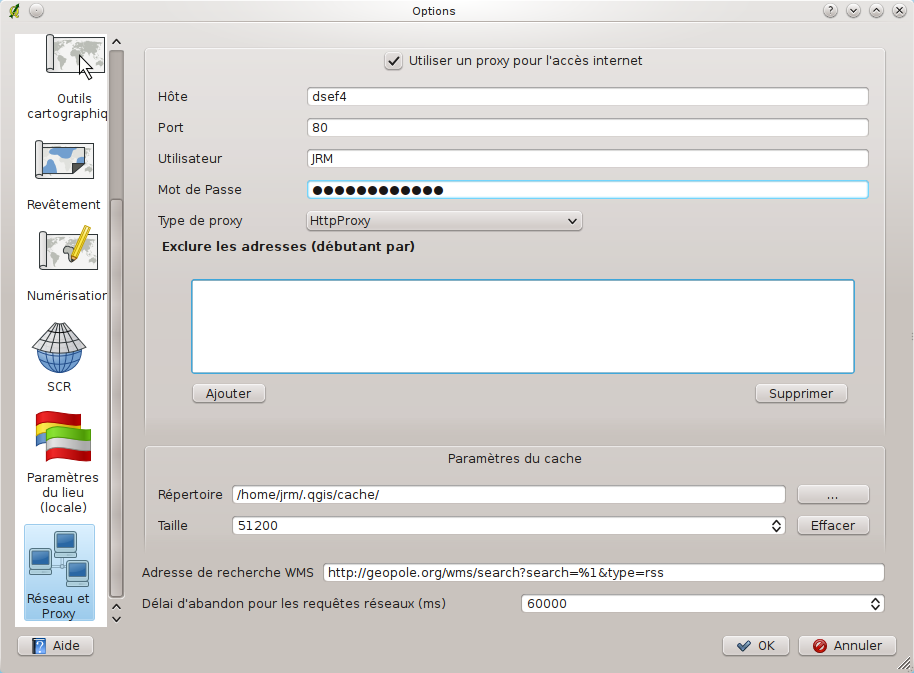
\includegraphics[clip=true, width=10cm]{proxy-settings}
   \label{fig:proxy-settings}
\end{center} 
\end{figure}

\begin{Tip} \caption{\textsc{Utilizzo dei proxy}}
\qgistip{L'utilizzo dei proxy può a volte essere complicato. E' utile testare 
i tipi di proxy succitati e controllare il loro funzionamento nel vostro caso specifico.
}
\end{Tip}

Queste opzioni possono essere modificate in funzione delle specifiche
esigenze. Alcuni cambiamenti potrebbero rendere necessario riavviare QGIS
prima che divengano attivi.

\begin{itemize}
\item \nix{Le impostazioni sono salvate in un file di testo: \$HOME/.config/QuantumGIS/qgis.conf}
\item \osx{Le impostazioni vengono collocate in: \$HOME/Library/Preferences/org.qgis.qgis.plist}
\item \win{Le impostazioni vengono inserite nel registro di sistema alla voce:}
\begin{verbatim}
\\HKEY\CURRENT\USER\Software\QuantumGIS\qgis
\end{verbatim}
\end{itemize}


\subsection{Segnalibri geospaziali}\label{sec:bookmarks}
\index{segnalibri}
\index{segnalibri geospaziali|\see{segnalibri}}

I segnalibri geospaziali consentono di "memorizzare" una posizione
geografica alla quale ritornare in un secondo momento.

\subsubsection{Creazione di un segnalibro}
Per creare un segnalibro:
\begin{enumerate}
\item Usare lo zoom o muovere la mappa all'estensione d'interesse.
\item Selezionare la voce di menu \mainmenuopt{Visualizza} >
\dropmenuopt{Nuovo segnalibro} o premere \keystroke{Ctrl-B}.
\item Inserire un nome descrittivo per il segnalibro (fino a 255 caratteri).
\item Cliccare su \button{OK} per aggiungere il segnalibro o \button{Cancel}
per uscire senza aggiungere il segnalibro.
\end{enumerate}

Si noti che è possibile avere più di un segnalibro con lo stesso nome.

\subsubsection{Uso e gestione dei segnalibri}
Per usare o gestire i segnalibri, selezionare la voce di menu
\mainmenuopt{Visualizza} > \dropmenuopt{Mostra segnalibri}.
La finestra \dialog{Segnalibri geospaziali} consente di usare lo zoom a un
segnalibro o di eliminarne uno.
Non è possibile editare il nome o le coordinate di un segnalibro.

\subsubsection{Zoom a un segnalibro}
Dalla finestra \dialog{Segnalibri geospaziali} dialog, selezionare il
segnalibro desidera cliccando su di esso, quindi cliccare su \button{Zoom a}.
Si può usare lo zoom su un segnalibro anche facendo doppio click su di esso.

\subsubsection{Cancellare un segnalibro}
Per cancellare un segnalibro dalla finestra \dialog{Segnalibri geospaziali},
cliccare su di esso e poi sul pulsante \button{Elimina}.
Confermare la scelta cliccando su \button{OK} o annullare l'eliminazione
cliccando su \button{Cancel}.
